\chapter{Религия}

\section{Научный атеизм: верить, не верить, как проверить?}

\textit{Источник: \url{https://4brain.ru/blog/nauchnyj-ateizm-verit-ne-verit-kak-proverit/}}

А давайте перенесемся в будущее, примерно в 2050 год, и попытаемся представить, как будут проходить уроки физики в школе через пару-тройку десятков лет? «Как идет ток по проводам? – С Божьей помощью! – Садись, пять!» Такой диалог ученика и учителя видится вполне реальным даже намного раньше, чем в 2050 году.

Разумеется, если только к этому времени физику не исключат из списка обязательных для изучения в школе предметов. После приказа Министерства просвещения, коим из перечня обязательных исключены астрономия, экономика, экология и право, удивляться не приходится ничему [Официальный интернет-портал правовой информации, 2022].

В том числе тому, что ракеты падают, вместо того, чтобы лететь, куда их направили. Взлетела, ударилась о небесный свод, упала, куда придется – что здесь непонятного? Так, видимо, будут объяснять все недоработки ракетной промышленности в обозримом будущем, когда знания по астрономии окончательно перейдут в категорию рудиментарных.

Наших читателей, уже прошедших программы «Критическое мышление» и «Когнитивистика», вряд ли чем-то можно сбить с толку. Мы приглашаем всех желающих присоединиться к нашему образовательному марафону, изучать наши программы и читать наши статьи. И наша сегодняшняя тема – научный атеизм.

\textbf{Что такое «научный атеизм»?}

Согласно существующему определению, научный атеизм – это система научно-материали- стических взглядов, основанная на полном отрицании существования Бога и прочих сверхъестественных сил.

Наличие явлений, не поддающихся трактовке с позиций науки, научный атеизм объясняет недостаточным уровнем развития научных знаний, который, впрочем, постоянно растет.

Следовательно, со временем все не вполне понятные на сегодняшний день явления будут изучены, поняты и все это без необходимости привлечения Божественных и других сверхъестественных субстанций.

\textbf{Научный атеизм: небольшой исторический экскурс}

Слово «атеизм» пришло к нам из далекой Античности. В древнегреческом языке слово atheos (читается как «атеос») означает «безбожный». Как мы понимаем, коль скоро слово с таким значением появилось в языке, значит, в социуме существовало такое явление, и возникла необходимость каким-то образом отобразить это в существующей системе обмена информацией.

Из известных мыслителей прошлых веков до нашей эры в существовании Бога очень сомневался Протагор (490-420), а Диагор Мелосский (475-410) и Феодор Киренский (340-250) прямо отрицали существование Бога. Термин atheismos («атеизм») использовал в своих работах Цицерон (106-43). С развитием научных знаний стали предприниматься попытки обосновать атеистические воззрения с научной точки зрения. Так зародилось понятие «научный атеизм».

Проследить эволюцию этого термина можно в книге Histoire de la littérature ancienne et moderne («История древней и современной литературы»), впервые изданной в 1829 году и восстановленной и переизданной уже в наступившем третьем тысячелетии [F. Schlegel, W. Duckett, 2011]. Уточним, с древних времен дошло не так много литературных источников, и в 19 веке древнюю литературу изучали без жесткого разделения на художественную и философскую.

В странах Западной Европы научный атеизм в большей степени приобрел форму научного скептицизма – подхода, согласно которому, все утверждения, которые не могут быть доказаны опытным путем, должны быть подвергнуты сомнению. А вот в нашей стране научный атеизм стал орудием идеологической борьбы, пропаганды и обработки массового сознания в нужном для партии направлении.

Да, в нашей стране риторика атеизма обязана своей распространенностью, массовым использованием и частым употреблением партийным лидерам ушедшей эпохи. Владимир Ленин, «вождь мирового пролетариата», создатель Российской социал-демократической рабочей партии (сокращенно РСДРП), впоследствии трансформировавшейся в РКП(б), ВКП(б) и затем в КПСС, рассматривал атеистическое воспитание как необходимую составляющую построения нового общества.

Его научные работы многократно переиздавались уже после его смерти, в частности, в виде сборника статей об атеизме, религии и церкви [В. Ленин, 1980]. В этих работах можно проследить формирование начал теории отражения и научного атеизма. Ленин писал, что отражение в сознании, образ представляет собой органическое единство непосредственного восприятия и прошлых впечатлений, объективного и субъективного, формы и содержания. В его понимании теория отражения как бы «соединяет» познающий субъект с познаваемым объектом и обеспечивает объективность научного познания, поэтому никакой необходимости в «божественном» объяснении окружающего мира не существует.

Собственно термин «научный атеизм» в СССР обрел популярность с началом правления Никиты Хрущева. Одно за другим вышли постановления «О крупных недостатках в научно-атеистической пропаганде и мерах по ее улучшению» и «Об ошибках в проведении научно-атеистической пропаганды среди населения». Уточним, что ранее в партийных руководящих документах использовался термин «антирелигиозная пропаганда», и лишь в 50-е годы было решено отказаться от противопоставления посредством приставки «анти» в пользу термина «научно-атеистическая пропаганда».

С 1959 года в высших учебных заведениях начали преподавать «Основы научного атеизма», сначала факультативно и не везде [М. Смирнов, 2018]. Но дело быстро набирало обороты, и уже в 1960 году научный атеизм в МГУ преподавали на всех факультетах. За столицей «подтянулась» вся страна, практически во всех вузах появилась кафедра научного атеизма. Появилась и соответствующая учебная литература. В частности, «Научный атеизм» учебник СССР для высших учебных заведений [А. Окулов, 1978].

В 1964 году был создан Институт научного атеизма, просуществовавший вплоть до развала СССР и еще какое-то время в уже переименованном виде как Институт религиоведения. Институт научного атеизма на протяжении почти всего своего времени существования выпускал сборник «Вопросы научного атеизма», в задачи которого, как было заявлено, входила разработка актуальных проблем теории и практики научного атеизма, анализ и обобщение опыта научно-атеистического воспитания.

Под эгидой общества «Знание» в рамках проекта «Новое в жизни, науке, технике» издавалась подписная научно-популярная серия «Научный атеизм» с упором в большей степени на историю и философию. В рамках этой серии вышла, к примеру, очень познавательная книга «Атеистические традиции в русской философии» [А. Сухов, 1989].

Показательно, что советские разработки в этом направлении вызывали определенный интерес в научных кругах на Западе. Так, в периодическом издании Studies in Soviet Thought («Исследования советской мысли») вышла статья Scientific Atheism: An Introduction («Научный атеизм: введение») [T. Blakeley, 1964].

Позднее вышла еще одна статья этого же автора под названием Marxist‐Leninist scientific atheism («Марксистско-ленинский научный атеизм») [T. Blakeley, 1966]. Автор делится своими выводами, что в его понимании главная цель марксистско-ленинского «научного атеизма» состоит в открытии и усвоении «научных» данных и использовании их в «атеистическом» уничтожении религии и всех ее придатков. Первая задача состоит в том, чтобы показать, используя данные преимущественно естественных наук, отсутствие объекта религии – Бога. Во-вторых, «научный атеизм» стремится объяснить, как возникла и продолжает проявлять признаки жизнестойкости теория без объекта, ищет причины или «корни» религии.

В нашей стране печатные издания на тему атеизма «сошли на нет» еще до распада Советского Союза. Было ли дело только в невостребованности и неактуальности темы в новых условиях перестройки и гласности или решающую роль сыграла нехватка финансирования, мы сейчас не узнаем. С учетом того, что в конце 80-начале 90-х недофинансирование ощущали даже весьма важные для обороноспособности страны отрасли, можно предположить, что финансовый фактор стал решающим.

Однако и тему востребованности тоже нельзя сбрасывать со счетов. Когда появляется актуальный запрос, находятся и ресурсы для его реализации. Примером может служить книга Устина Чащихина «Научный атеизм» (скачать можно здесь) вышедшая в 2013 году спустя более чем 20 лет после того, как Советский Союз канул в Лету. А в 2022 году вышла новая книга, которую написал Устин Чащихин «Научный атеизм – спасение России».

Что это за актуальность такая с учетом того, что в российских школах уже давно преподается Закон Божий под красивым названием «Основы православной культуры»? А вот об этом стоит поговорить подробнее.

\textbf{Научный атеизм сегодня: актуально или нет?}

На самом деле, поводов обратить взор в сторону научного атеизма сегодня более чем достаточно. Судите сами: церквями и храмами у нас застроили все вокруг, детишек сызмальства заставляют изучать Закон Божий, сами все молимся и крестимся, чуть ли не двумя руками, а живем все хуже и хуже. И ладно бы дело было только в материальной составляющей.

Зла и ненависти стало вокруг намного больше, невзирая на то, что религии и морали, вроде как, все пути к нашим сердцам открыты. А заповедь «Не убий», такое впечатление, что все просто позабыли и действуют строго наоборот, особенно в 2022 году.

Люди постарше вполне могут вспомнить, что в эпоху марксизма-ленинизма, научного атеизма и научного коммунизма военные конфликты, если и возникали, решались исключительно \ed{усилиями}{усилие}{effort} действующей армии и без особой \ed{огласки}{огласка}{publicity}. Митинги и демонстрации были исключительно праздничные, приуроченные к различным «красным дням календаря» и, естественно, санкционированные властью.

И, что характерно, особых поводов хотя бы задуматься о несанкционированном митинге протеста не было. Это не к тому, что «раньше было лучше», а к тому, что с проблемами, которые есть всегда и в любом государстве, каким-то образом справлялись так, чтобы не нарушать покой «широких народных масс».

Так может, если перестать молиться и начать думать, а вместо храмов и церквей строить школы и университеты, все как-то наладится? Знать это однозначно и заранее невозможно, однако повод задуматься, безусловно, есть.

Ранее упомянутая нами книга «Научный атеизм» начинается с той ценной мысли, что, если Бог не может уничтожить зло, значит, он не всемогущ, а если не хочет, то его доброта, мягко говоря, сильно преувеличена [У. Чащихин, 2013].

Если же Бог не может и не хочет уничтожить зло, тогда зачем он вообще такой нужен? Эту мысль когда-то высказал древнегреческий философ Эпикур (342-271), однако тема актуальна по сей день. Видимо, за добротой и \ed{человеколюбием}{человеколюбие}{philanthropy} – это точно не в церковь.

Вышеупомянутое издание «Научный атеизм» – книга, которая содержит много отсылок к историческому материалу. Автор очень настаивает на том, чтобы люди, считающие себя верующими, внимательно прочитали «Ветхий Завет» и «Новый Завет» и задумались, что именно они взяли за образец в своей жизни.

Все подряд цитировать не будем, однако то, что в библейской литературе много чего такого, что к доброте и человеколюбию не имеет никакого отношения, это факт. Просто цитата: «И послал тебя Господь в путь, сказав: иди и предай заклятию нечестивых Амаликитян и воюй против них, \explain{доколе не уничтожишь их}{until you destroy them}» [allbible, 2015].

При всем понимании, что у каждой фразы есть свой контекст, сложно смириться, что призыв решить проблему военным путем \explain{из уст}{from the mouth} Господа – это нормально. Так что религия – это не так однозначно хорошо, как это пытаются внушить на уровне государства, которое, вроде как, отделено от церкви.

Почему тогда научный атеизм времен СССР так и не прижился в массовом сознании, невзирая на то, что его преподавали в вузах, пропагандировали посредством научно-популярной литературы, а ночному пасхальному богослужению всегда предлагали более \ed{зажигательную}{зажигательная}{incendiary} альтернативу – концерт Аллы Пугачевой и других звезд \ed{эстрады}{эстрада}{stage} по центральному телевидению?

Автор книги «Научный атеизм» объясняет это не слишком высоким профессиональным уровнем тогдашней научно-атеистической пропаганды [У. Чащихин, 2013]. По сути, тогда в подготовке материалов по научному атеизму в полную силу участвовали представители только одной науки – философии, а аргументы из естественных наук были на уровне школьных учебников физики, географии и биологии.

Сам автор явно гордится тем, что он не гуманитарий, а представитель естественных наук, что уже само по себе должно обеспечить более современную и «\ed{продвинутую}{продвинутая}{advanced}» аргументацию. Зачем нужна эта аргументация и зачем в принципе опять поднимать на щит вопросы научного атеизма?

А вот с этого момента появляется ощущение, что где-то мы уже это все видели, слышали, читали и проходили. Ответ на вопрос «Зачем нужен научный атеизм» сводится к следующим постулатам:
\begin{enumerate}
    \item Научный атеизм развивает научное мышление.
    \item Научный атеизм экономит время, которые верующие тратят на молитвы и посещение церкви.
    \item Научный атеизм экономит денежные средства, которые верующие тратят на покупку церковной атрибутики.
    \item Научный атеизм прекращает религиозные войны и религиозную ненависть.
\end{enumerate}

\ed{Насчет}{насчёт}{as regards} последнего можно поразмыслить. Быть может, если дать «ИГИЛовцам» (признана в РФ экстремистской организацией) почитать книжки по научному атеизму, что-то и изменится. А вот насчет экономии времени и денег – вряд ли это станет весомым аргументом, который может сподвигнуть верующих отказаться от веры и соблюдения церковных ритуалов. Эти же аргументы – экономия времени и денег – можно выдвинуть желающим «собраться с ребятами на пиво», «сходить с девочками попить кофе», «поехать порыбачить на русалок» и т.д.

Гипотетически в этой жизни можно не тратиться ни на что, кроме еды, жилья, одежды и средств гигиены, только что это будет за жизнь? Прихожане любой церкви – это почти как участники группы по интересам, где у каждого своя интенсивность участия в общем деле. Кто-то посещает церковь по всем праздникам, скупает все свечки, причащается и исповедуется, а кто-то приходить лишь на Рождество и Пасху и довольствуется ролью зрителя.

Так за что же борется или «против кого дружит» научный атеизм? То, что Бог, даже если он есть, не всесилен и не может решить проблемы людей без их участия понятно даже глубоко верующим. Как говорится, батюшка в бронежилете и бронированном джипе – наглядное подтверждение известной поговорки «На Бога надейся, а сам не плошай».

\begin{center}
    
\includegraphics[width=0.8\textwidth]{img/holy-water.jpg}
\end{center}

Так ли далеко от этого ушел научный атеизм – карикатуры, которые использовались для научно-атеистической пропаганды, говорят об обратном. Например, для того, чтобы святая вода исправно поступала верующим, нужен исправно работающий водовод, а для того чтобы его отремонтировать, нужен водопроводчик.



Есть и еще одна вариация на эту тему, когда заболевший священнослужитель обращается со словами «Помоги, Господи» к аптекарю, а не собственно к Богу.

Что и чему здесь противоречит? Маловероятно, что священнослужители возьмутся оспаривать необходимость вызвать сантехника, если сломался водовод, или обратиться к врачу в случае болезни, потому как «На Бога надейся, а сам не плошай». Или вот такой опус:

\begin{fancyquotes}
    У церковного порога ждешь, поп, напрасно:\\
    Без икон и Бога мы живем прекрасно!
\end{fancyquotes}

Как говорится, слава Богу, что кто-то может решить свои проблемы своими силами и не беспокоить Всевышнего всякими мелочами:

\begin{wrapfigure}{l}{0.5\textwidth}
    
\includegraphics[width=0.5\textwidth]{img/atheism-church.jpg}
\end{wrapfigure}
Иначе может получиться, как в анекдоте, когда глубоко верующий попал и постоянно молившийся прихожанин в ад, а крепко пьющий столяр-безбожник – в рай. На вопрос верующего «Почему?» последовал вполне логичный ответ, что где это видано, чтобы табуретки бегали за столяром и «доставали» его своими проблемами.

\begin{wrapfigure}{r}{0.5\textwidth}
    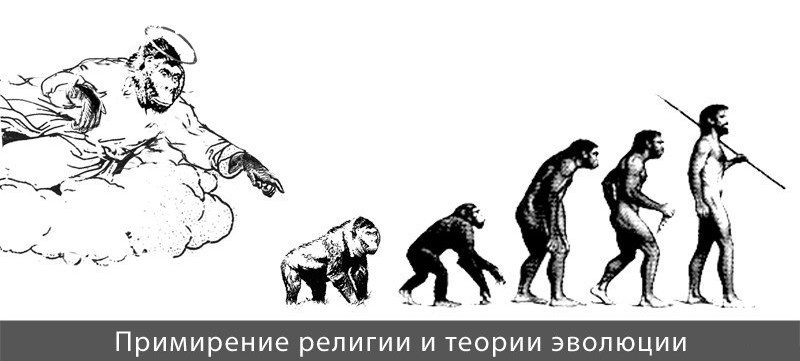
\includegraphics[width=0.5\textwidth]{img/atheism-monkey.jpg}
\end{wrapfigure}
Были, правда, и попытки «примирения» науки и религии, к примеру, по вопросу о происхождении человека. С учетом того, что живьем Бога все равно никто не видел, допущения могут быть абсолютно любые. Насколько удачные – судите сами.
Однако самой фееричной на тему научного атеизма карикатурой можно считать, пожалуй, ту, где студентка молится Богу, чтобы сдать научный атеизм:

Как говорится, «кафедра научного атеизма в шоке», но кого это волнует, когда «на кону» стипендия.

Так или иначе, и в религиозной, и в научно-атеистической пропаганде можно найти какие-то изъяны. Однако есть ученые, которые занимаются критикой научного атеизма профессионально и получают за это зарплату.\\


\textbf{Критика научного атеизма}

Сегодня в обществе существует запрос на сохранение баланса между верой и знанием, светским и религиозным, охрану личных границ от вмешательства какой-либо идеологии со стороны будь то церкви или государства. Именно этим и обусловлены циклические всплески интереса к вопросам научного атеизма.

Однако у определенной группы ученых есть большие сомнения, что научный атеизм может решить эту задачу и что в принципе в ныне существующем виде научный атеизм имеет право называться научным. Так, в статье The reasons for «scientific» atheism (Причины «научного» атеизма) можно найти витиеватую мысль насчет того, что «научный атеизм противоречит сам себе, потому что, если бы он был правдой, ему не пришлось бы трудиться, чтобы опровергнуть иллюзию» [J. Cañizares, 2012].

Стоит ли это понимать так, что если бы география была правдой, так ей бы не пришлось опровергать иллюзию многих поколений людей, что Земля плоская? А если бы правдой была химия, то ей не пришлось бы опровергать иллюзию божественного происхождения молекул и атомов, и в химических формулах и таблице Менделеева не было бы никакой необходимости? Как говорится, «не совсем понятно».

\begin{wrapfigure}{l}{0.5\textwidth}
    
\includegraphics[width=0.48\textwidth]{img/atheism-4.jpg}
\end{wrapfigure}
Есть и более здравые мысли. Бразильский физик-теоретик Марсело Глейзер в своем интервью по поводу получения Темплтоновской премии 2019 года заявил, что «отсутствие доказательств не является доказательством отсутствия», и именно поэтому «атеизм несовместим с научным методом» [L. Billings, 2019].

Насчет того, что «отсутствие доказательств не является доказательством отсутствия», с этим нужно полностью согласиться. Однако само по себе «отсутствие доказательств отсутствия» не может автоматически считаться доказательством присутствия. В этом плане атеизм полностью следует в русле формы научного скептицизма – подхода, согласно которому, все утверждения, которые не могут быть доказаны опытным путем, должны быть подвергнуты сомнению.

Всем, кому хочется больше критики, можем порекомендовать статью «Сердце бессердечного мира: Как родился и умер советский научный атеизм» [А. Коняев, А. Артемьев, 2013]. Мы долго останавливаться на критических замечаниях не будем ввиду однотипности предлагаемых критиками аргументов и бессмысленности критики всего, что в какой-то момент времени оказалось востребованным и отвечающим запросам текущей ситуации.

В конце концов, религия – это не только идеология, которую можно принимать или не принимать, критиковать или продвигать в массы. Это красивые обряды, это душевные песнопения, это самобытная архитектура церквей. Это еще несколько праздников в наш насыщенный трудовыми буднями календарь, это возможность отдохнуть душой, отмечая вместе с близкими людьми, к примеру, Пасху.

Подготовка к этому празднеству столь же замечательна, как и само празднование: покраска яиц всей семьей, выбор узоров и красящих субстанций, эксклюзивные сюжеты и стандартные трафареты, которые нужно максимально гармонично разместить на поверхности яйца. А в день Пасхи по традиции принято устраивать «сражения», по очереди ударяя друг о друга окрашенные куриные яйца и выясняя, с какой стороны скорлупа крепче: с более округлой или с более заостренной.

Большинство людей, отмечающих Пасху и красящих куриные яйца, не читали Библию и не считают для себя обязательным посещение церкви. Стоит ли им мешать просто наслаждаться жизнью, праздниками, общением и застольем, досаждая всяческими опусами на тему научного атеизма и ненужности религии как таковой?

Думается, вряд ли, потому что у нас уже была страна, которая пыталась запрещать людям совершать церковные обряды, крестить детей и венчаться, праздновать Пасху, читать Солженицына и Довлатова, слушать «Битлз» и ДДТ. Страна называлась СССР, и ее больше нет, в то время как книги Солженицына и Довлатова читают до сих пор, «Битлз» и ДДТ как слушали, так и слушают, а Пасху как отмечали, так и будут отмечать дальше все, кто считает это нужным для себя.

Закончит так же плохо, как СССР, любая другая страна, которая будет запрещать, ограничивать и убеждать людей в том, что им не нужно многое из того, к чему они привыкли? Мы не знаем, но проверять не хотелось бы. А хотелось бы, чтобы в нашу жизнь вернулся мир, добро и взаимопонимание, причем совершенно не важно, как: через религию, науку или атеизм.

\newpage
\section{Язык и религия}

\textit{Источник: \url{https://4brain.ru/blog/jazyk-i-religija/}}
Религию можно обозначать в любых категориях – ее называют системой верований, идеологией, «опиумом», неосознанным и трансцендентальным знанием об окружающем мире. В любом виде она представляет сначала систему идей, концепций, ассоциаций и сравнений, которые могут переноситься людьми в материальную культуру.

Но, независимо от категорий, важно понимать одно: религия без слов, общего языка и системы мышления не сможет существовать больше одного поколения. Религия – это совокупность неких абстрактных смыслов, которые можно передать при помощи слов, языка.

В идеализированном понимании религия не предусматривает необходимости защищать себя от скептиков или же искать самой себе подтверждения – передачи знания и религиозных основ от поколения к поколению было бы достаточно, чтобы последователи поддерживали религию живой. Подходящей цитатой в этом случае является цитата Джалаладдин Руми (Sufi mystic Rumi): «Тишина – это язык Бога».

Но с другой стороны, исторически становится очевидным, что язык как средство сохранения религии является также и главной причиной, почему религиозные знания не могут передаваться дословно, точно, без интерпретаций, скептицизма и дискурсивности. Именно создавая новые интерпретации той или иной догмы, множество скептиков или реформистов создавали новую религию.

Таким образом, вопрос связи языка и религии – это нечто больше, чем сохранение культурной традиции. Язык и религия вызывают интерес разных мыслителей и ученых на протяжении столетий, начиная со времен Аристотеля и заканчивая сегодняшним днем (больше о последних исследованиях можно почитать в нашей статье «Язык и мышление»).

\textbf{Обозначение взаимозависимости}

С философской точки зрения, язык и религия – это два инструмента человеческого сознания, которые помогают объяснить организацию внешнего мира, создать ощущение общности. Поэтому религия и язык являются такими же формами сознания, как философия, мораль, право, искусство и наука, ибо все они преследуют единую цель – отображать мир в сознании человека.

Поскольку язык и религия – это два разных подхода к пониманию мира, для более четкого обозначения предмета дискуссии их используют вместе, как понятие «язык и религия». Это придает новое значение данным понятиям и позволяет рассматривать их наряду с другими стойкими философскими категориями, такими как «язык и общество», «язык и сознание», «язык и культура».

Но все-таки очевидным можно назвать то утверждение, что религия является более зависимой от языка. Именно при помощи языка создаются и сохраняются все религиозные образы, что делает психологические структуры языка и религии между собой тесно сплетёнными.

\textbf{Вильгельм фон Гумбольдт и «дух народа»}

Интерес к изучению истории и духа (культуры) европейских народов был заложен философом Вильгельмом фон Гумбольдтом. Вслед за философией Гегеля, который провозгласил идею «духа народа» неотъемлемой составной частью человеческого бытия, Гумбольдт развил направление сравнительной антропологии, которое интересовалось историей, бытом, фольклором и, конечно же, религией – важными составными чертами народов.

Непосредственно Гумбольдт также предположил, что язык возник как результат духовного развития народа, и это нечто большее, чем общественное сознание, – это различное видение мира. К такому заключению он пришел во время изучения языка басков, который разительно отличался от языков своей индоевропейской семьи. В своей работе «О различии строения человеческих языков и его влиянии на духовное развитие человечества» Гумбольдт описывал непосредственное влияние языка на формирование духовного сознания человека.

\textbf{Сакрализация текстов и их роль}

Наивысшей формой развития духовного сознания некой общности людей является создание собственных сакральных книг – Торы, Священного Писания, Корана, Авесты, проповедей Будды. Каждый из этих текстов стал чем-то большим, нежели просто послужил формированию народной общности, – со временем приверженцы той или иной религии не ограничивались географическими границами, могли сохранять чувство единения с единомышленниками независимо от местонахождения. Такое чувство общности оказалось даже более стойким в формировании ментального родства, чем использование одного языка, на котором тексты были написаны.

Таким образом, независимо от религии и языка, на котором передаются сакральные знания, язык и религия все равно являются важными элементами человеческого познания и объяснением мироустройства, роли человеческой жизни и жизни после смерти.

Другая важная особенность сакральных текстов состоит в том, что вокруг них формируется целая прослойка важных культурных и духовных проявлений приверженцев – особое религиозное мироощущение, традиции, обряды, религиозная мораль, религиозные институты. Все эти материальные проявления абстрактной религии делают более четкими и понятными духовную практику для многих последователей вне национальных ограничений.

\textbf{Атеистический экзистенциализм: возможна ли жизнь без Бога}

Несмотря на силу религиозного учения и его интерпретации общественного строя, другим проявлением человеческого сознания является полное или частичное отрицание божественной, мифической и духовной потребности человека в Боге в любой форме – трансцендентальной, метафизической и религиозной. Приверженцы этого философского направления – атеистического экзистенциализма (Жан-Поль Сартр, Альбер Камю, Мартин Хайдеггер и Симона де Бовуар), опровергая большинство принятых христианских канонов, не смогли выйти из религиозной перспективы мира, ибо заявили о реинкарнации как форме спасения.

\textbf{Религиозная практика сегодня}

В современном мире, транскультурные границы которого все больше и больше теряют свое значение, святость религиозного языка выглядит, как последний не тлеющий бастион. Особенно в мегаполисах или в далеких странах религия и язык часто являются самыми важными атрибутами национального и культурного единства. Молитва на родном языке сохраняет ощущение единства с культурой и историей.

В современном глобальном мире, где люди часто теряют свои корни и помнят о них из детских рассказов, изучение родного языка и молитва на нем выполняют важную практику духовного воссоединения со своими корнями. Такая тенденция наиболее популярна среди современного еврейского населения, часть которого проживает в разных странах мира. Именно язык и религия являются источниками воссоединения с прошлым. Для них иврит – это интимный способ понимания своей религии, культуры и философии в более точных понятиях. Таким образом, независимо от контекста, именно использование религиозных терминов в ежедневном лексиконе, вместе с отмечанием праздников, помогает осмысливать свое существование и историю.

С другой стороны, разнообразный исламский мир именно при помощи религиозного языка и канонов веры сохраняет свое ощущение единства – из 5 разновидностей арабского языка сиро-палестинский диалект (Levantine Arabic) – самый универсальный, и на этом диалекте написан Коран, поэтому он понятен большинству арабов.

И более того, язык религии может не только поддерживать существование национальной культуры, где бы ее последователи ни обитали, – он может создавать новые общества, объединяя разных людей. Именно такой необычный путь свойственен классическому тибетскому языку. Его первые последователи появились в Британии в 1960-х гг., где учредили монастырь и стали объединять всех желающих изучать буддизм.

\textbf{Вместо заключения}

Язык и религия как мировоззрение являются проявлением человеческого сознания, и, независимо от трансформаций, служат неотъемлемым способами познания мира человеком. Их роль заключается в более сложной функции, чем роль общественного или политического мировоззрения, ибо при помощи религии и языка человечество пытается не столько обустроить свою жизнь, сколько найти ответы на вопросы о своем существовании.